\documentclass{article}
\usepackage{graphicx} %package to manage images
\usepackage[utf8]{inputenc}
\usepackage[a4paper, total={6in, 8in}]{geometry}
\usepackage{xurl}
\title{Relatório 5 \\ Pré-processamento}
\author{Pedro A. S. O. Neto}
\date{Fevereiro 2022}

\begin{document}

\maketitle

\section{Aplicação do filtro}

O problema destacado no relatório 3 foi resolvido. As fixações de 8ms dizem respeito aos dados brutos, onde nenhum algorítmo é aplicado para classificar eye-events (i.e., sacadas/fixações).
Nós aplicamos o filtro I-VT, com todos os parâmetros default. Os gráficos abaixo representam os dados com o novo filtro.

Problema: nesses gráficos, eu estou tratando todas as fixações como fixações do mesmo tipo. Ou seja, não estou diferenciando entre fixações e sacadas. Precisamos discutir nossas motivações teórias para separar ou não separar os tipos de fixação.

\begin{figure}[t]
\caption{Abacaxi}
\noindent\makebox[\textwidth]{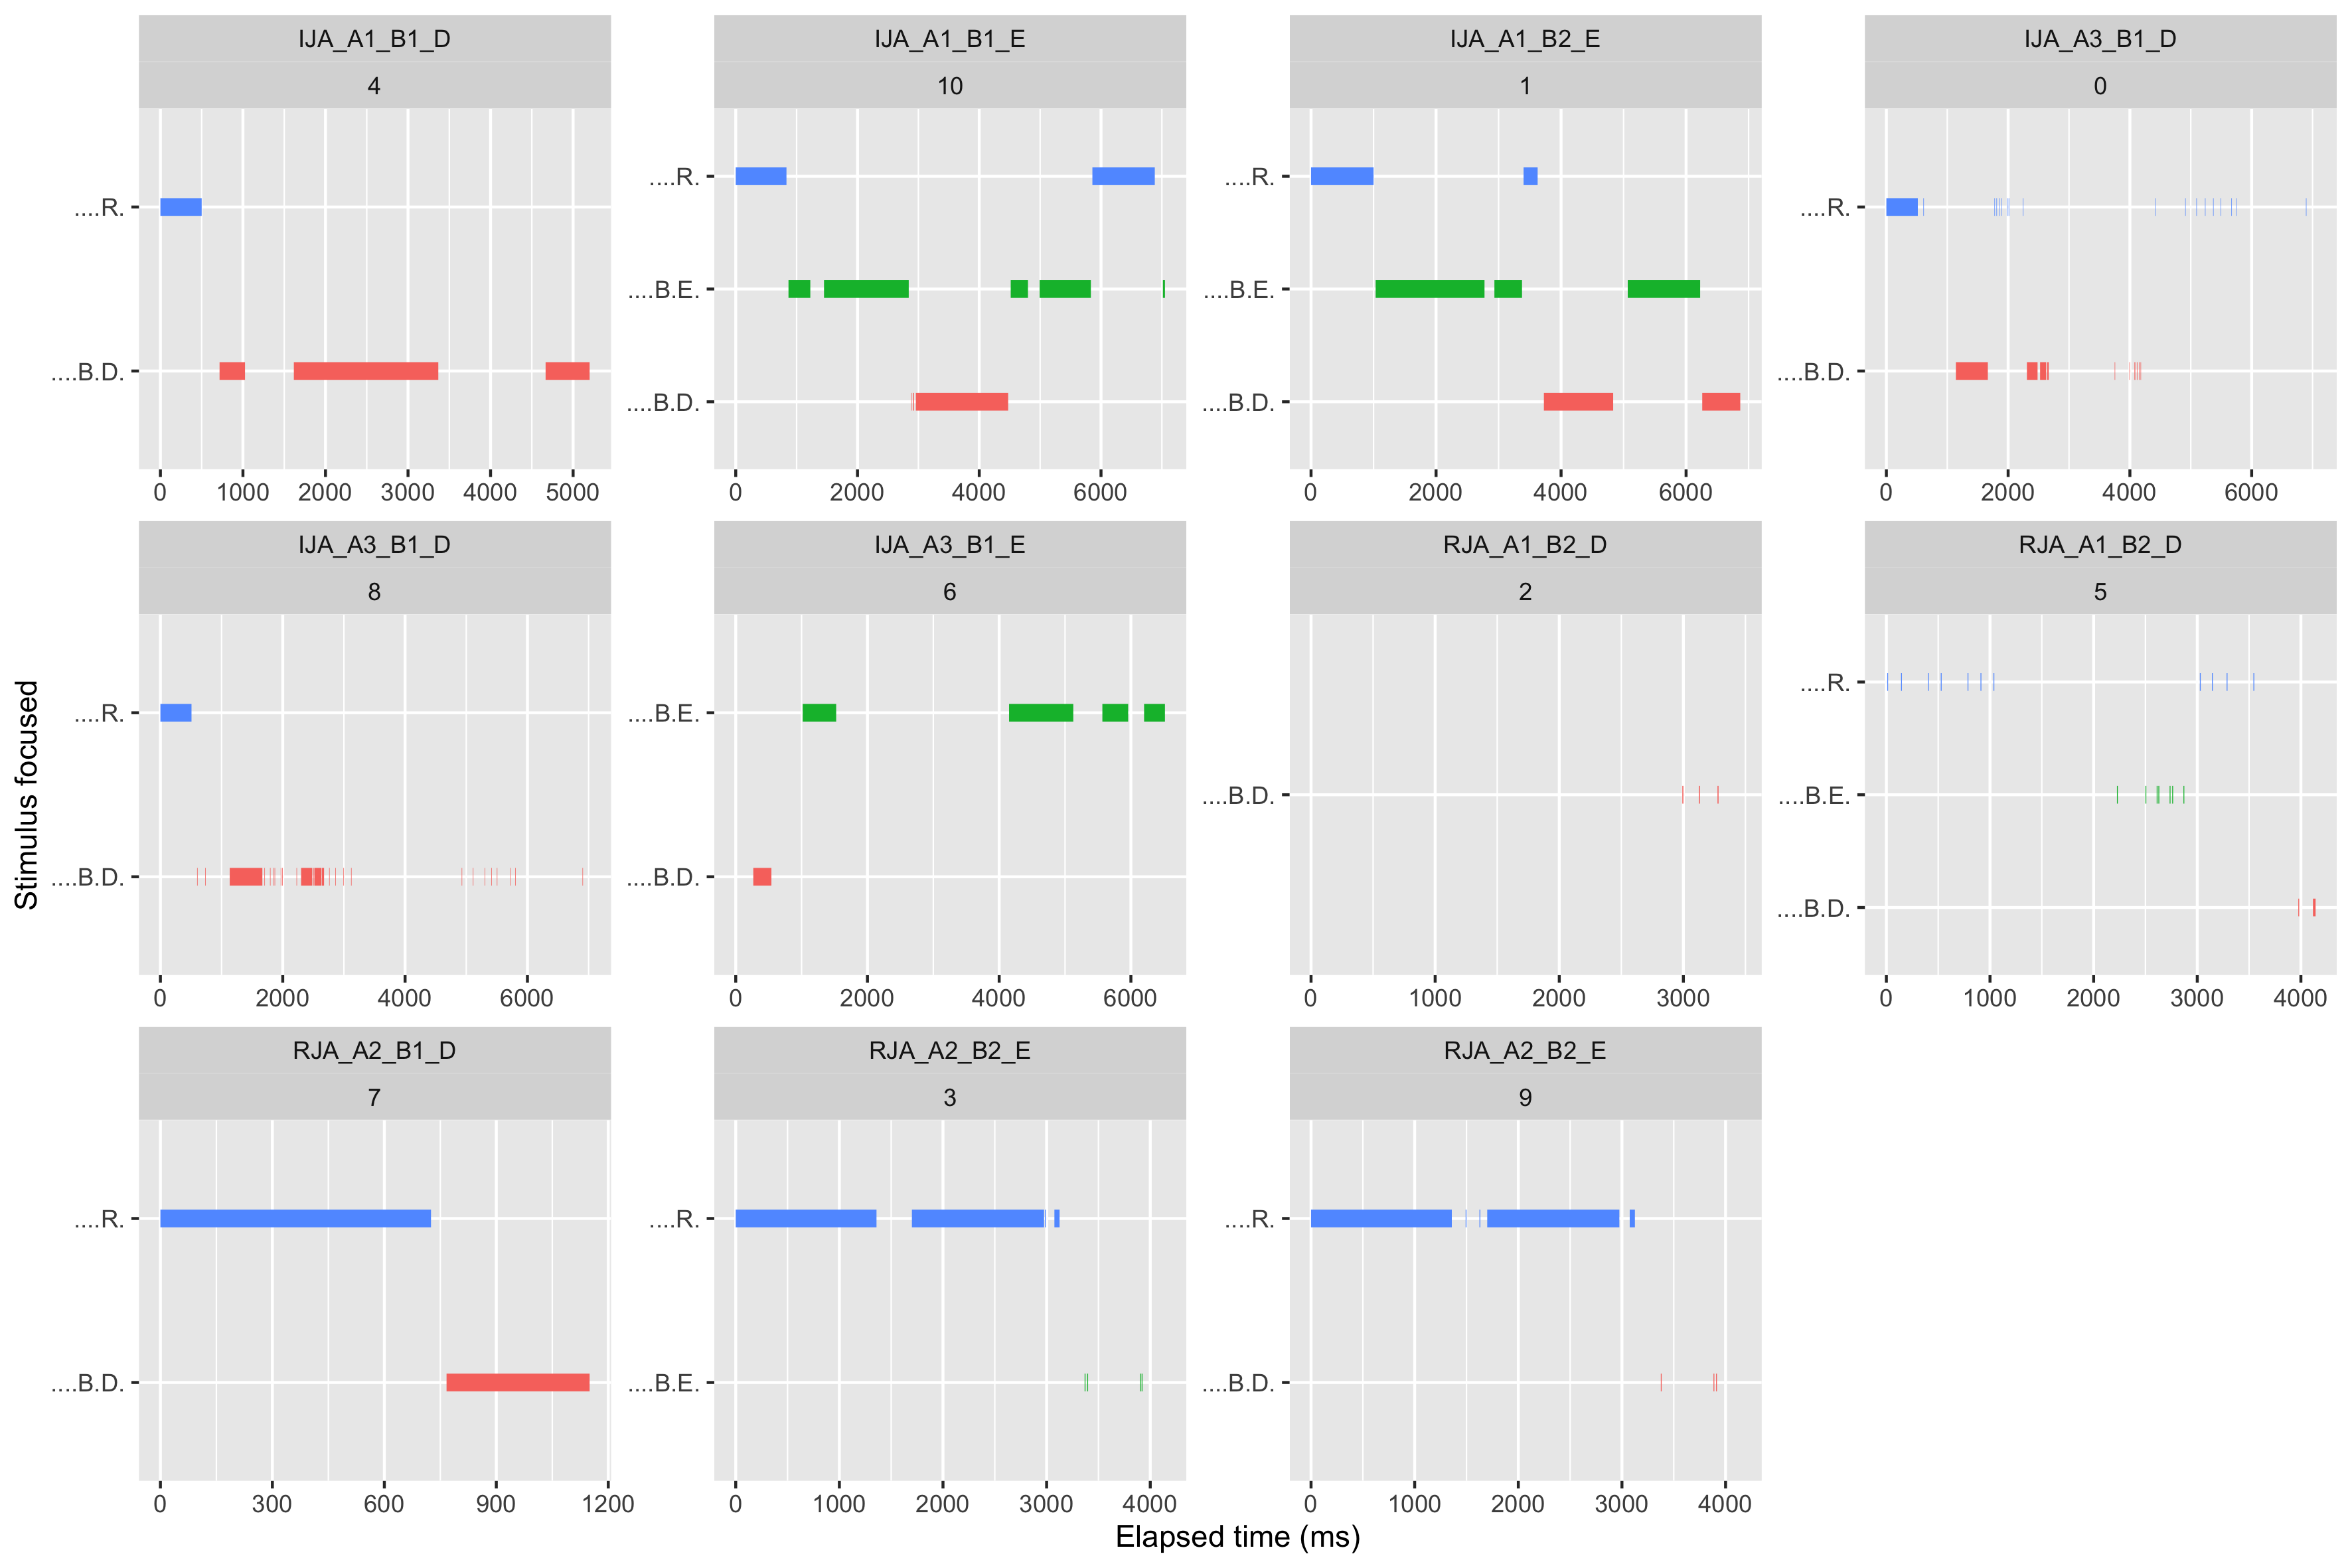
\includegraphics[width=\paperwidth]{"./graph_visu1.png"}}
\centering
\end{figure}

\begin{figure}[t]
\caption{Babacu}
\noindent\makebox[\textwidth]{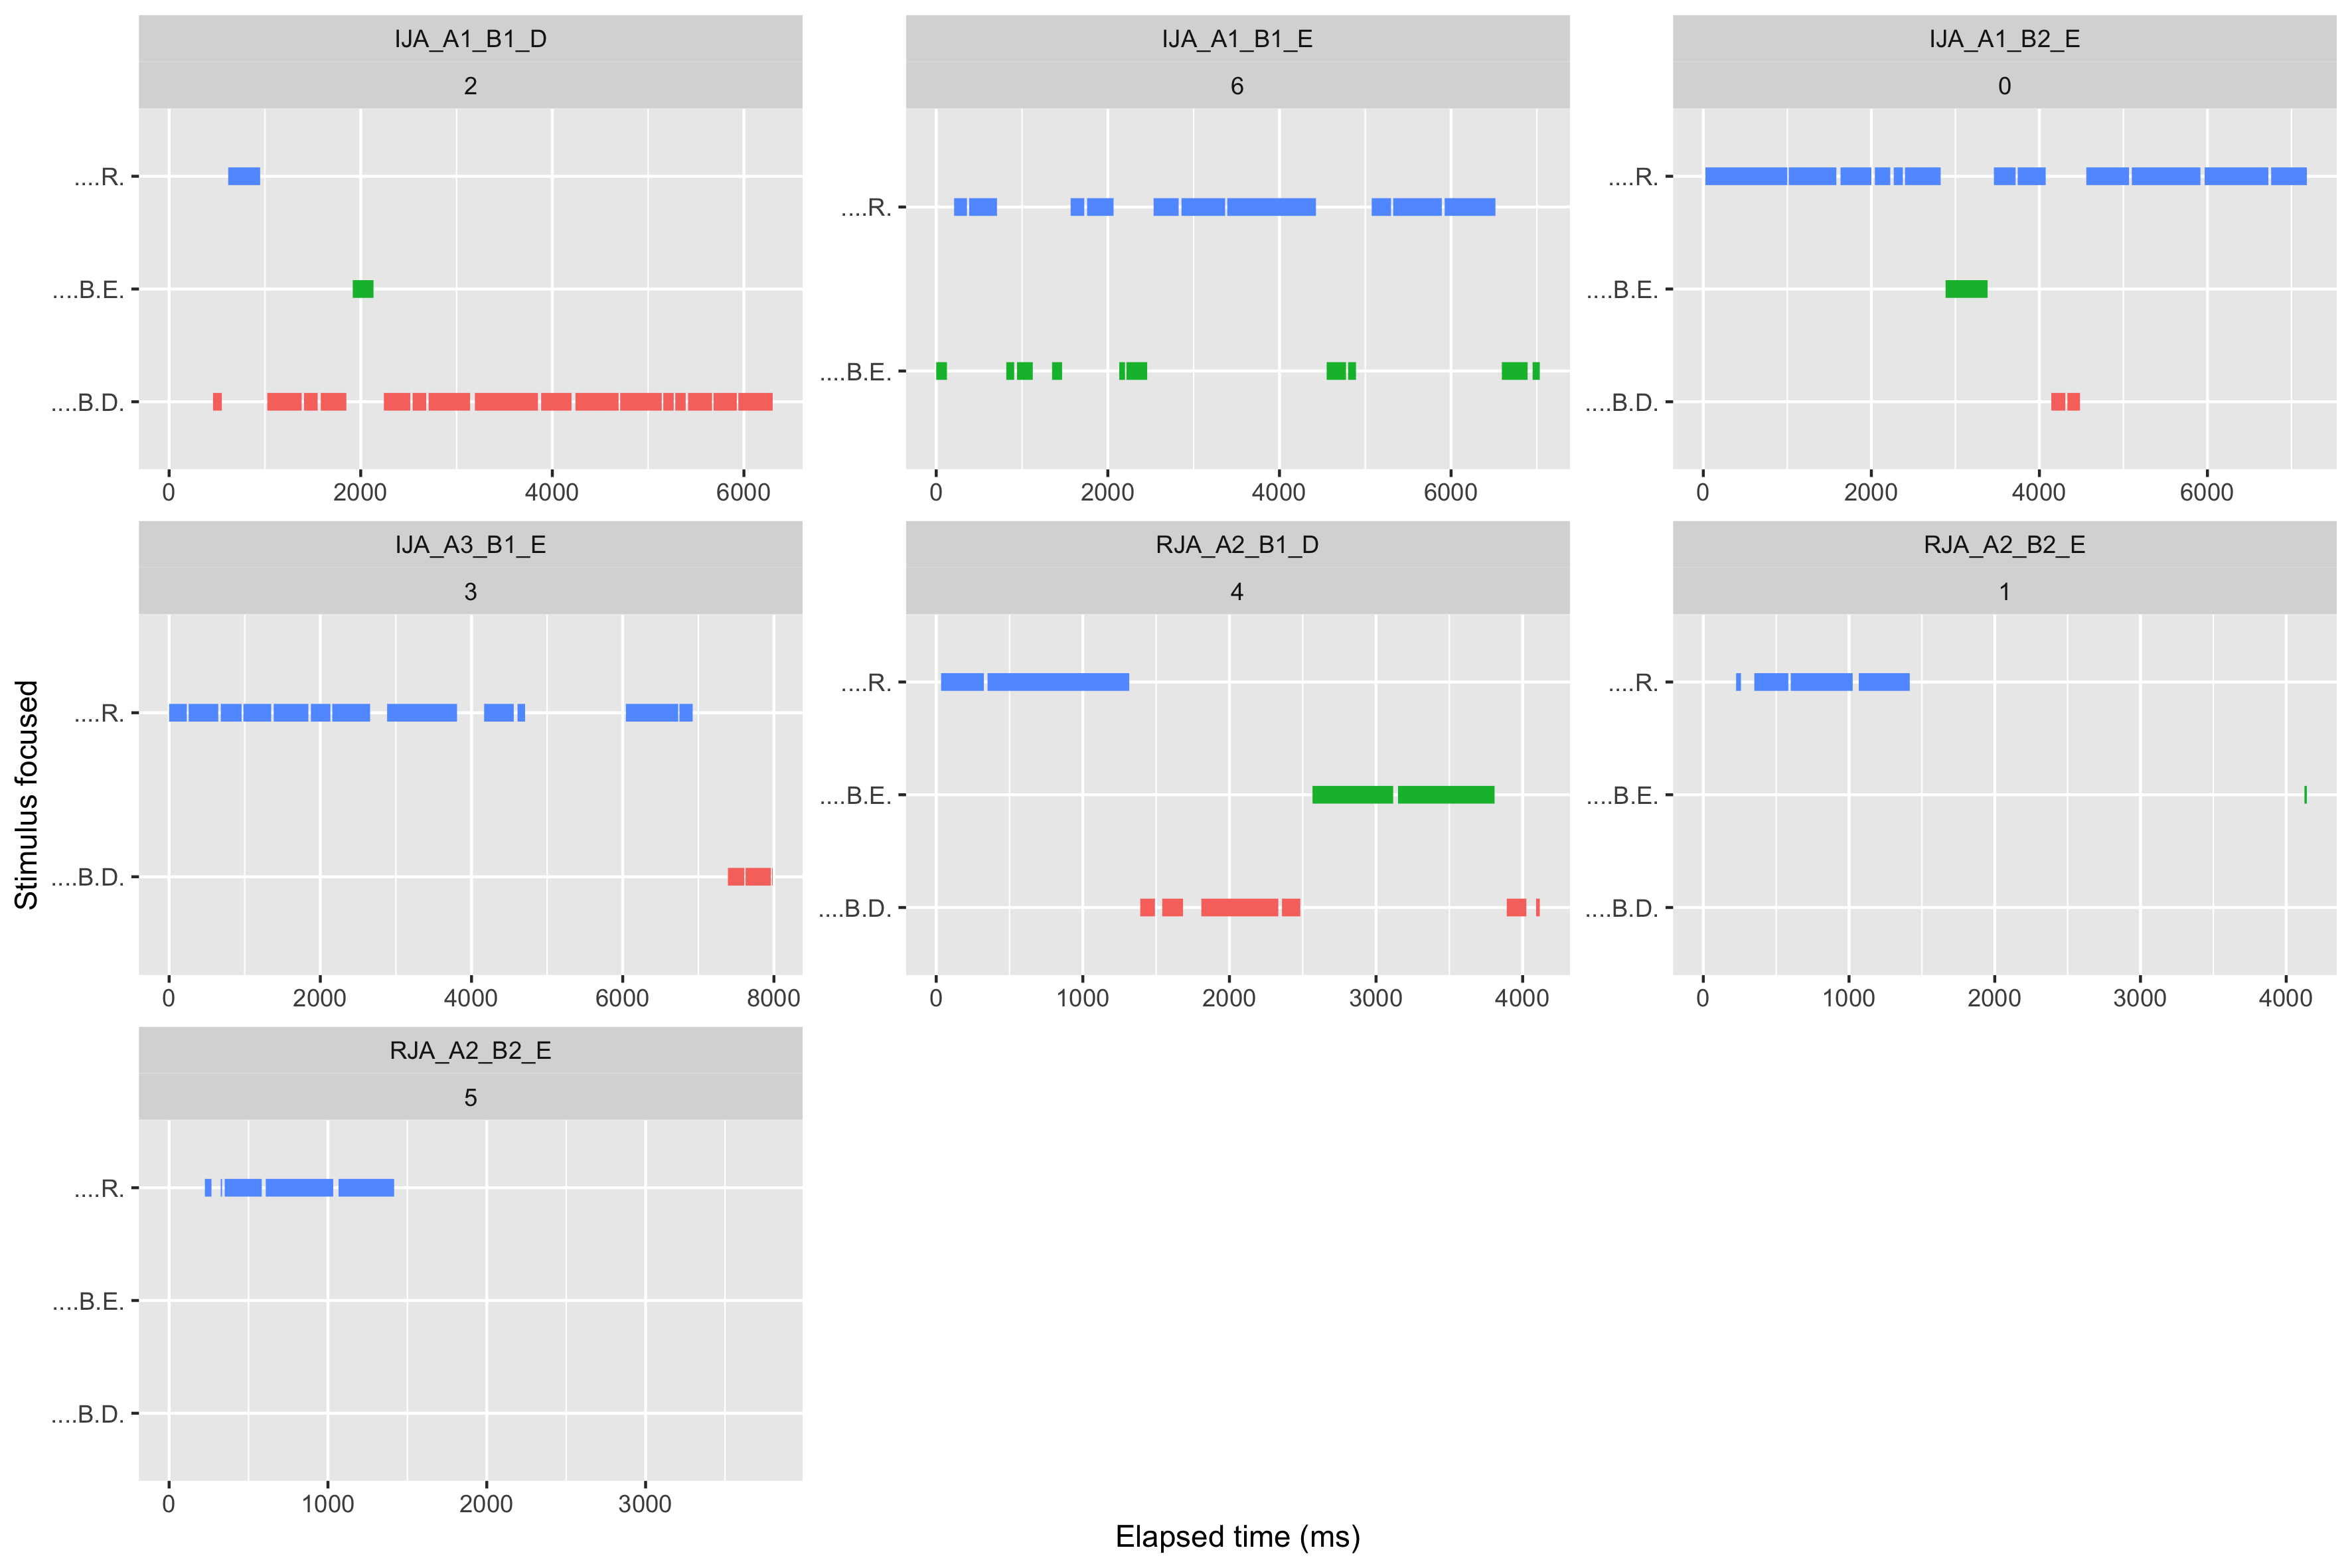
\includegraphics[width=\paperwidth]{"./graph_visu2.png"}}
\centering
\end{figure}

\begin{figure}[t]
\caption{Baru}
\noindent\makebox[\textwidth]{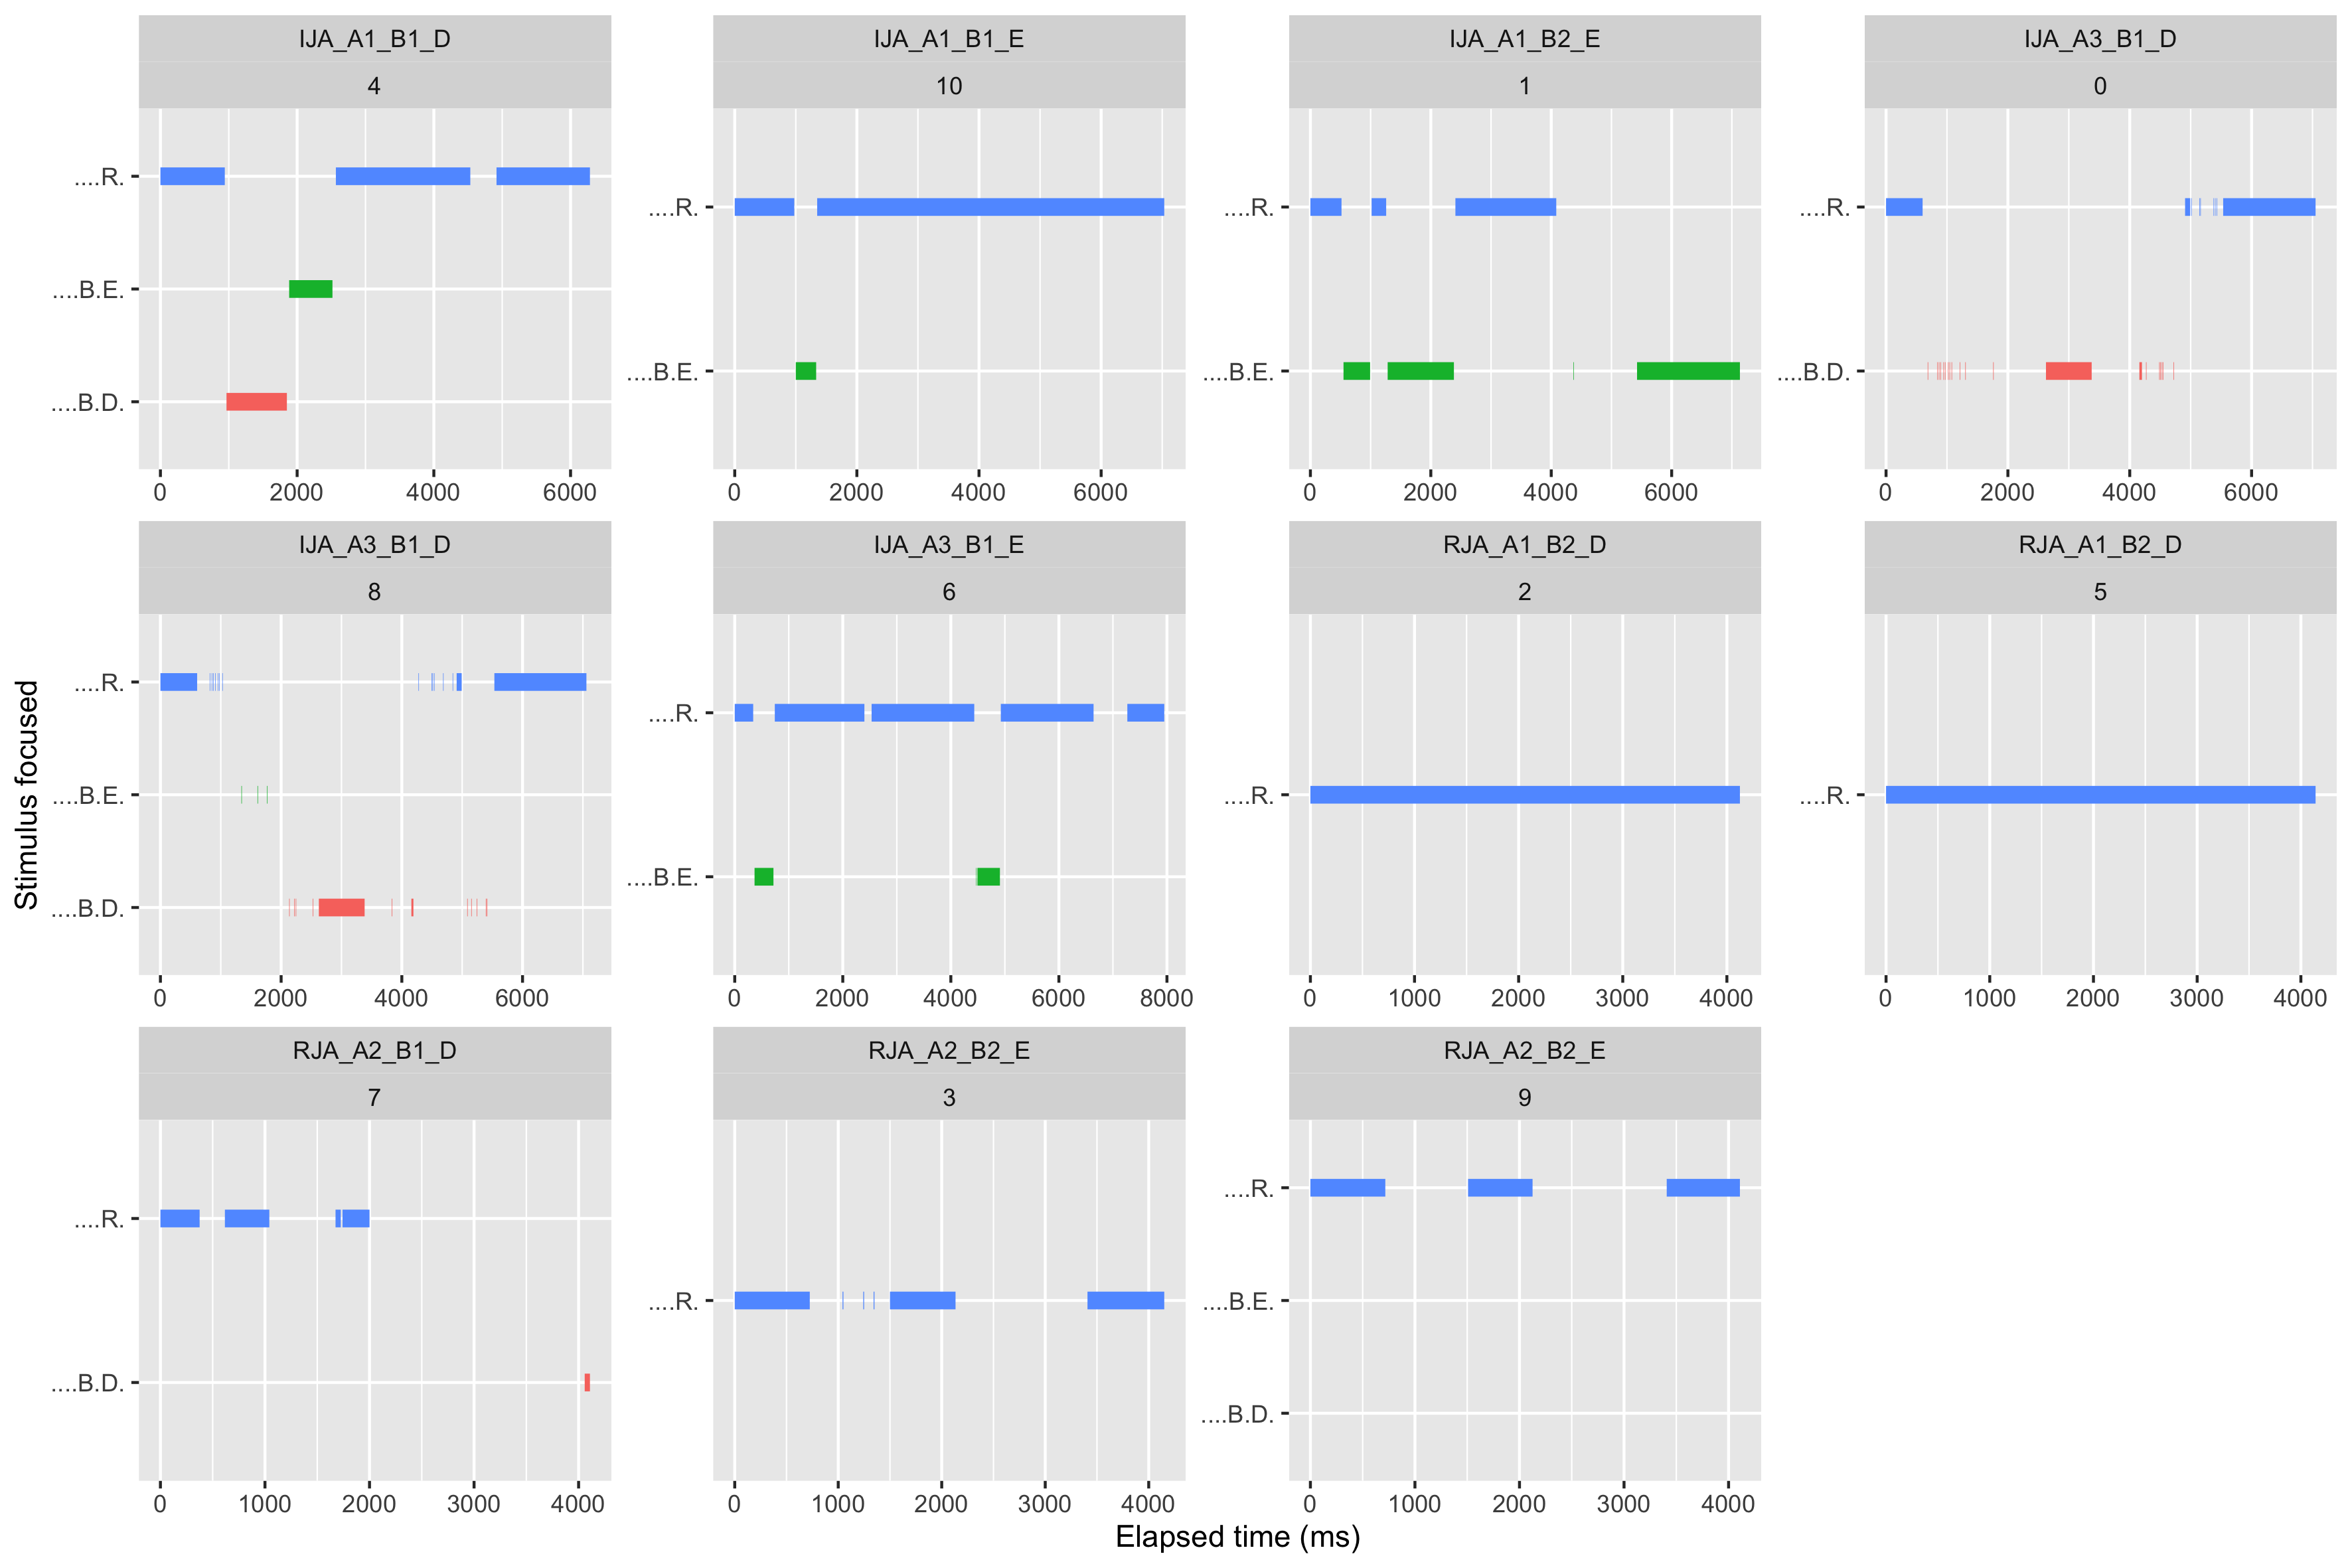
\includegraphics[width=\paperwidth]{"./graph_visu3.png"}}
\centering
\end{figure}

\begin{figure}[t]
\caption{Dovyalis}
\noindent\makebox[\textwidth]{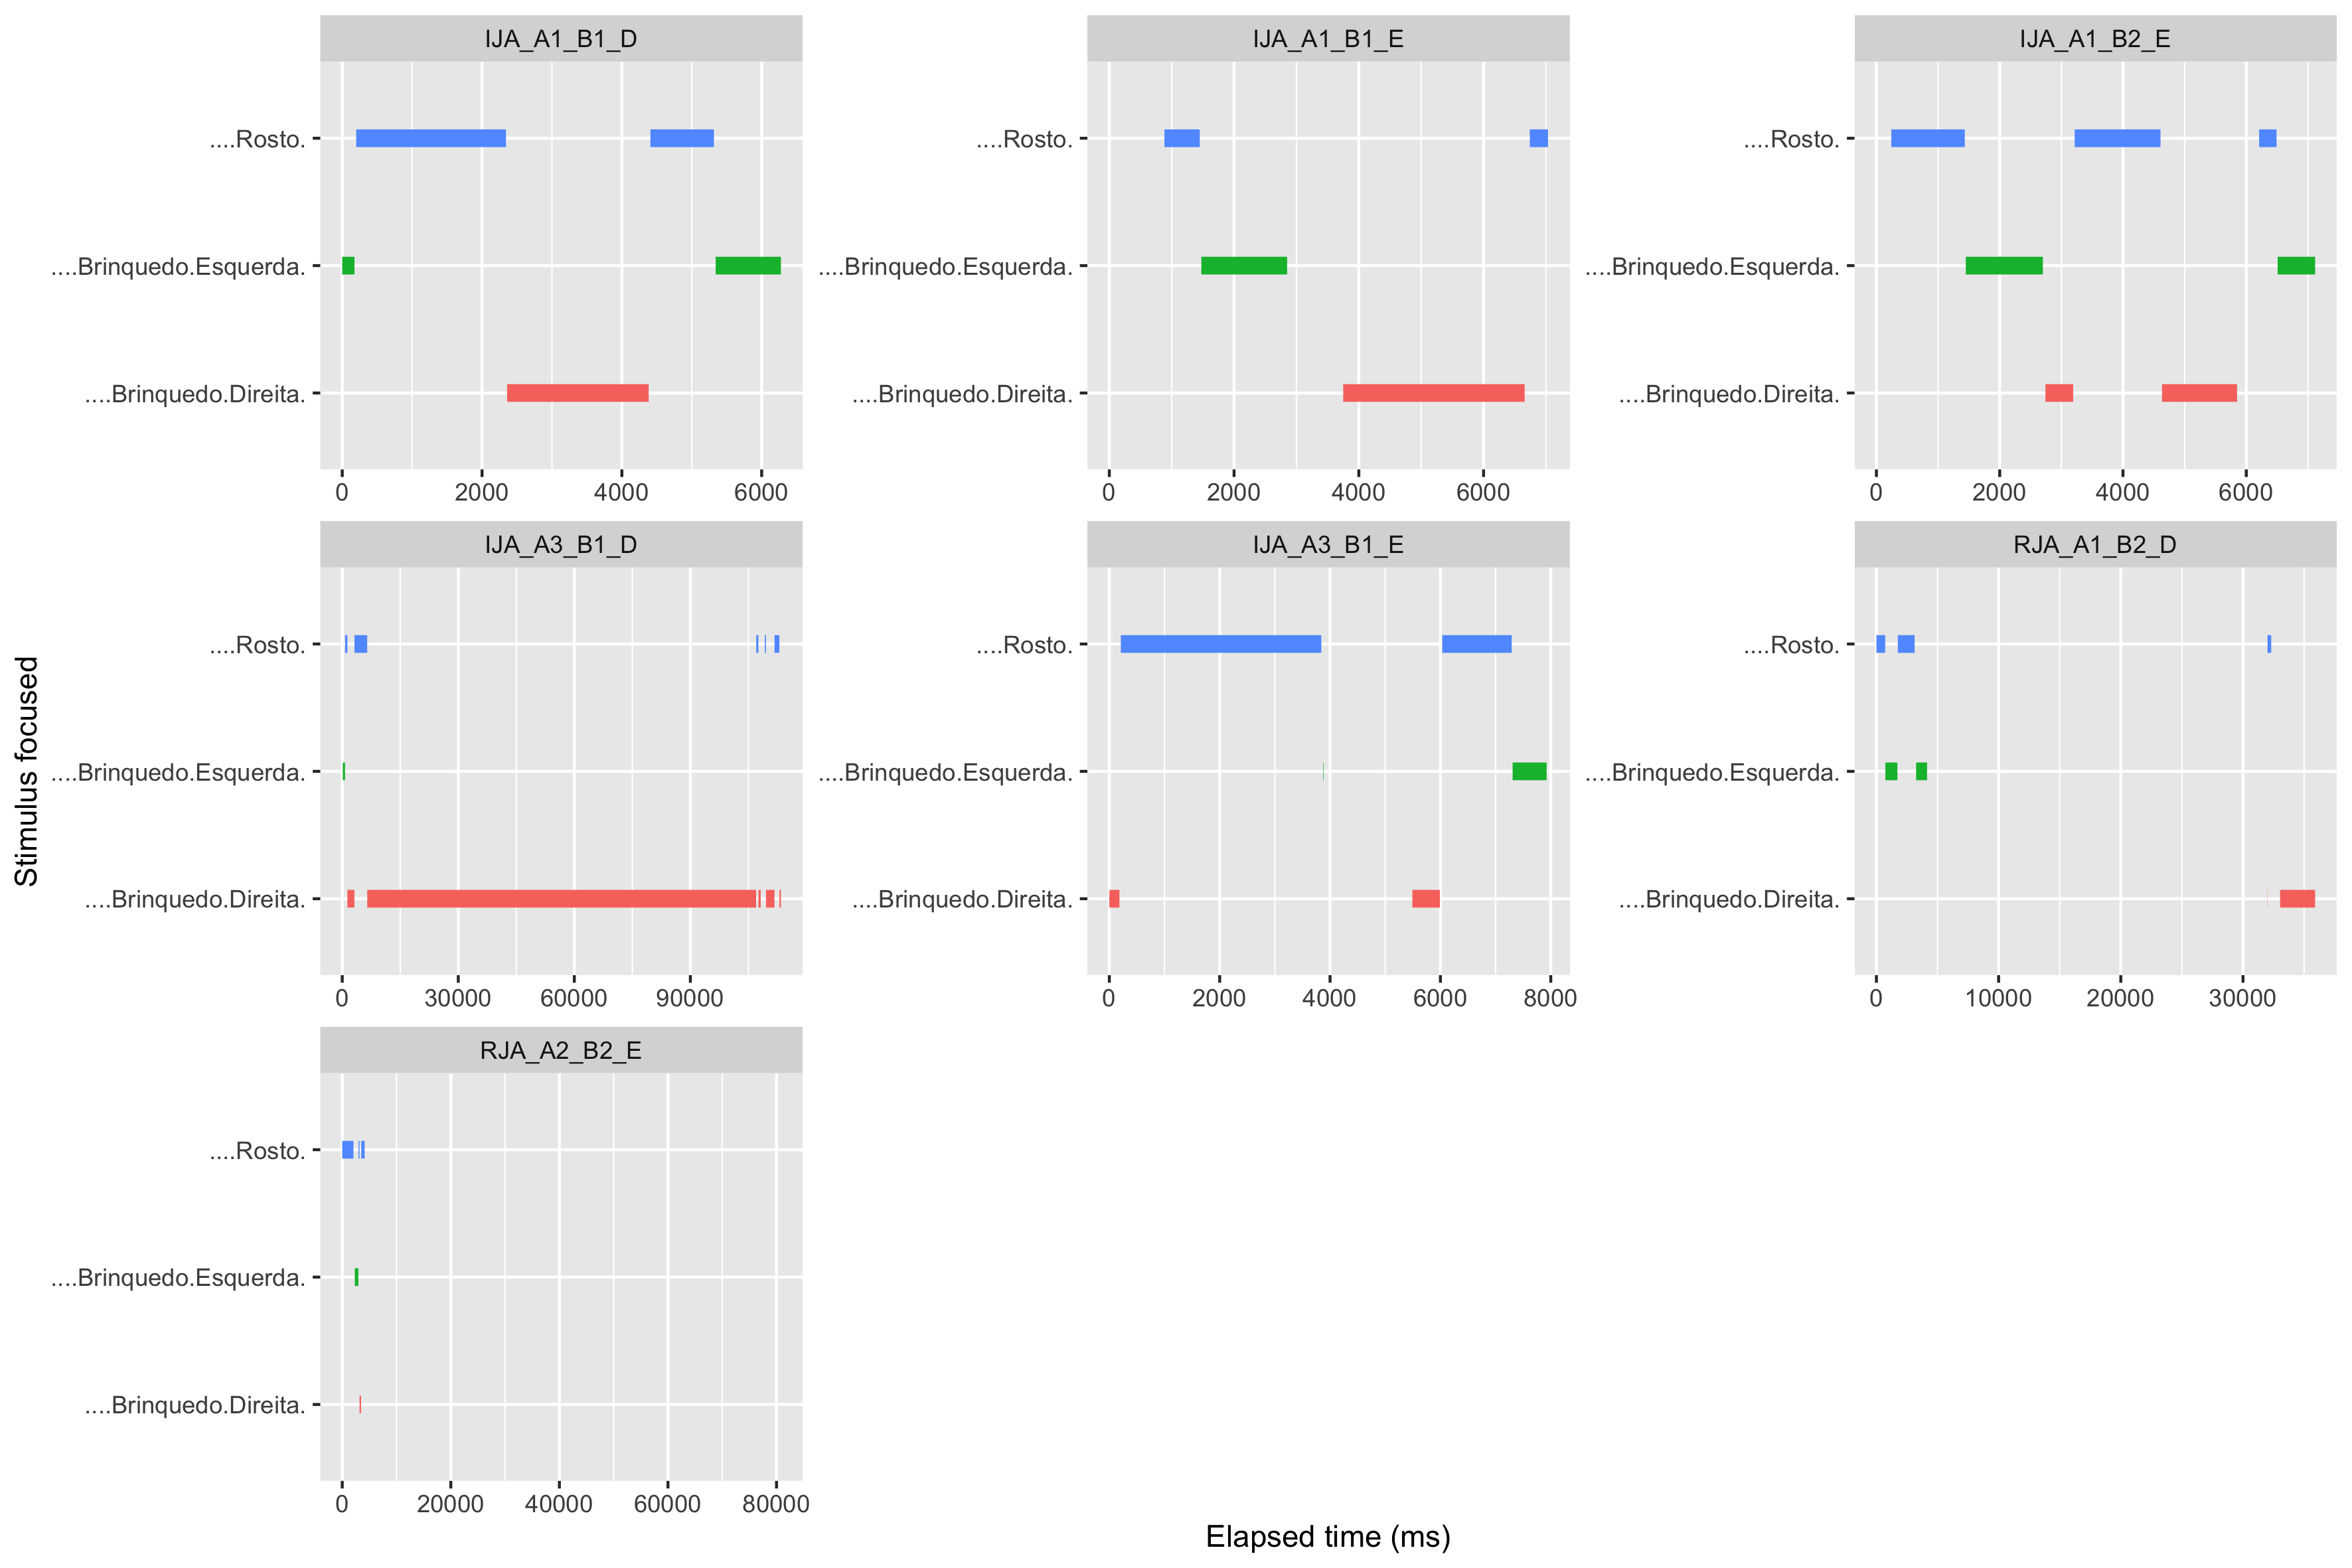
\includegraphics[width=\paperwidth]{"./graph_visu4.png"}}
\centering
\end{figure}

\begin{figure}[t]
\caption{Safira}
\noindent\makebox[\textwidth]{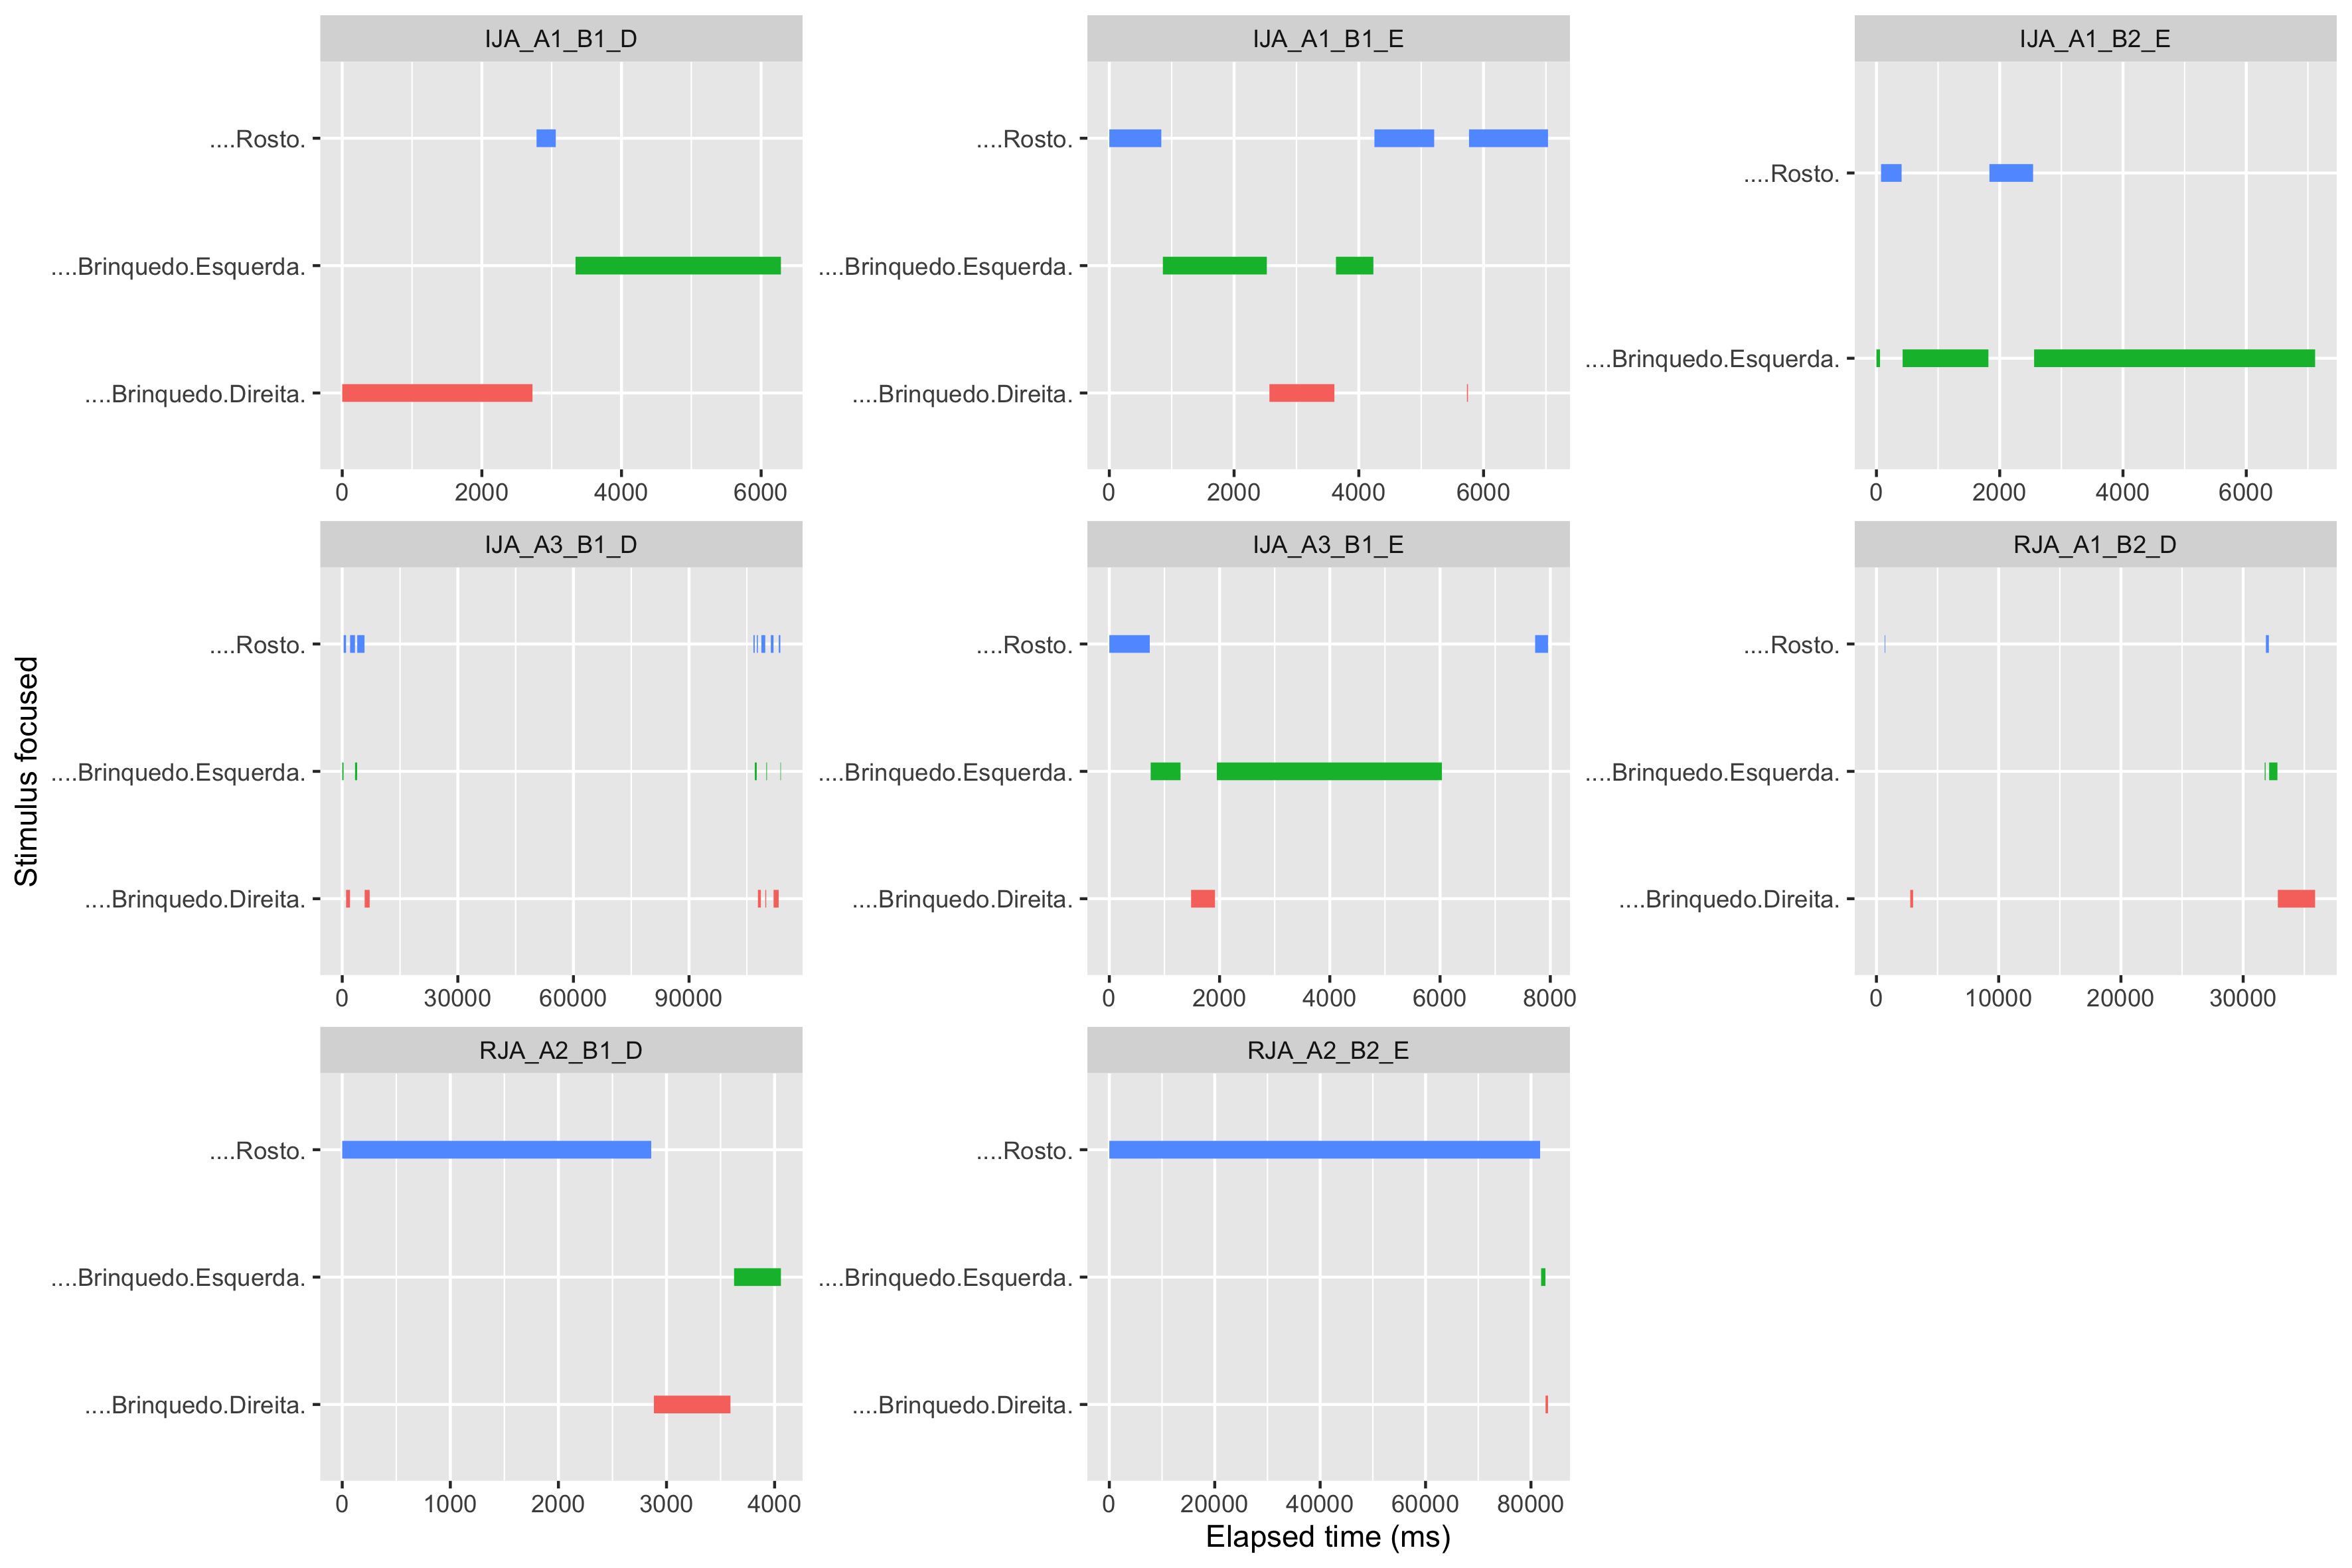
\includegraphics[width=\paperwidth]{"./graph_visu5.png"}}
\centering
\end{figure}

\end{document}


